\documentclass[a4paper,14pt]{extreport}
\usepackage[utf8]{inputenc}
\usepackage[T2A]{fontenc}
\usepackage[russian]{babel}
\usepackage{eufrak}
% поля:
\usepackage[left=1cm, right=1cm, top=2cm, bottom=2cm]{geometry}
\linespread{1}
\usepackage{indentfirst} % отделять первую строку раздела абзацным отступом
\setlength\parindent{5ex}
\addto{\captionsrussian}{\renewcommand*{\contentsname}{Содержание}}
\usepackage[hidelinks]{hyperref} % гиперссылки в содержании
\usepackage{graphicx}
\usepackage{float}
\usepackage{amsmath}
\renewcommand*{\thesection}{\arabic{section}}

\usepackage{multirow}
\usepackage[normalem]{ulem}
\useunder{\uline}{\ul}{}

\usepackage{cmap}%позволяет копировать кириллицу из скомпилированного файла

% Глубина разделов, попадающих в содержание
\setcounter{tocdepth}{3}

\linespread{1.3} % настройка межстрочного интервала
\tolerance=1000 % настройка чувствительности вставки переносов
\hfuzz=0pt
\sloppy

\begin{document}
	
	\begin{titlepage}
		\begin{center}
			\large
			МИНИСТЕРСТВО ОБРАЗОВАНИЯ И НАУКИ\\ РОССИЙСКОЙ ФЕДЕРАЦИИ
			
			\textbf{Федеральное агентство по образованию}
			\vspace{0.5cm}
			
			УНИВЕРСИТЕТ ИТМО
			\vspace{0.25cm}
			
			Факультет компьютерных технологий и управления
			
			Кафедра систем управления и информатики
			\vfill
			
			
			Студент: Артемов Кирилл\\
			группа P4135\\
			Вариант №2\\
			\textsc{Лабораторная работа №6}\\[5mm]
			
			{\LARGE Синтез дискретного устройства оценки полной размерности}
			\bigskip
			
		\end{center}
		\vfill
		
		\newlength{\ML}
		\settowidth{\ML}{«\underline{\hspace{0.7cm}}» \underline{\hspace{2cm}}}
		\hfill\begin{minipage}{0.4\textwidth}
			Преподаватель\\
			\underline{\hspace{\ML}} Ю.\,В.~Литвинов\\
			«\underline{\hspace{0.7cm}}» \underline{\hspace{2cm}} 2016 г.
		\end{minipage}%
		\bigskip
		
		\vfill
		
		\begin{center}
			Санкт-Петербург, 2016 г.
		\end{center}
	\end{titlepage}
	\newpage
	
	\section{Цель работы}
	
	Ознакомление с принципами построения дискретных устройств оценки полной	размерности.
	
	\section{Вариант задания}
		\begin{table}[H]
		\centering
		\caption{Параметры ОУ}
		\label{my-label}
		\begin{tabular}{|c|c|c|c|c|c|c|c|c|c|}
			\hline
			№ & ОУ & $k_1$ & $a_0^1$ & $T_1$ & $\xi$ & $k_2$ & $a_0^2$ & $T_2$ & T   \\ \hline
			2 & 1  & 1     & 0       & 0     & 0     & 0.5   & 1       & 0.95  & 0.5 \\ \hline
		\end{tabular}
	\end{table}
	
	\begin{figure}[H]
		\center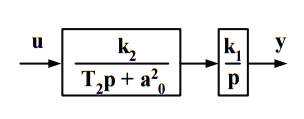
\includegraphics[width=0.5\linewidth]{oc.png}
		\caption{Объект управления}
		\label{fig:scr1}
	\end{figure}

	\section{Порядок выполнения работы}
	a) Синтез устройства оценки полной дискретной системы стабилизации
	
	В лабораторной работе No4 была разработана система стабилизации вид:
	\begin{equation}
	\begin{cases}
	\begin{bmatrix}
	x_1(k+1)\\
	x_2(k+1)
	\end{bmatrix} &=
	\begin{bmatrix}
	0&0.2859793\\
	0& 1.3010219
	\end{bmatrix}
	\begin{bmatrix}
	x_1(k)\\
	x_2(k)
	\end{bmatrix} + 
	\begin{bmatrix}
	0.0179897\\
	0.1505109
	\end{bmatrix}
	K_d 	
	\begin{bmatrix}
	x_1(k)\\
	x_2(k)
	\end{bmatrix}\\
	y(k) &= 
	\begin{bmatrix}
	1 & 0
	\end{bmatrix}
	\begin{bmatrix}
	x_1(k)\\
	x_2(k)
	\end{bmatrix}
	\end{cases}
	\end{equation}
	где матрица линейных стационарных обратных связей (МЛСОС):
	\begin{equation}
	K_d = 
	\begin{bmatrix}
	5.7748572    &6.4571995 
	\end{bmatrix}
	\end{equation}
	Заданный интервал дискретности:
	\begin{equation}
		T = 0.5 сек.
	\end{equation}
	Требуется синтезировать для (1) устройство оценки полной размерности (наблюдатель) вида:
	\begin{equation}
		\begin{cases}
		\hat{x} (k+1) = A_d \hat{x}(k) +L (y_u (k) - C_u \hat{x} (k)) + B_d u(k)\\
		u(k) = K_d \hat{x} (k)
		\end{cases}
	\end{equation}
	
	где $\hat{x} (k)$ -- вектор состояния устройства оценки полной размерности, 	$L - (l \times n)$ -- матрица входа устройства оценки полной размерности, $K_d$ -- матрица линейных стационарных связей.
	
	Разность между векторами состояния объекта управления и наблюдателя составляет вектор невязки:
	\begin{equation}
		\tilde{x} (k) = x(k) - \hat{x} (k)
	\end{equation}
	\begin{equation}
		\tilde{x} (k) = A_d \tilde{x} (k) - L C_u \tilde{x} (k) = F_z \tilde{x} (k)
	\end{equation}
	где $F_z = A_d - L C_u$ -- матрица замкнутой системы.
	
	Задача синтеза состоит в выборе такой матрицы входов $L$, чтобы
	собственные числа матрицы $F_z$ были по модулю меньше $1$.
	\begin{equation}
		z{F_z} \le 1
	\end{equation}

	Целью является сведение к нулю вектора невязки:
	\begin{equation}
		\tilde{x} (k) \mapsto 0
	\end{equation}	
	
	\subsubsection{Синтез наблюдателя}
	
	\begin{enumerate}
		\item 
		
		Для ОУ определитель матрица наблюдаемости равен:
		\begin{equation}
		Q_d =det
		\begin{bmatrix}
		1&    0\\         
		1 &   0.2859793  
		\end{bmatrix}
		=0.2859793  \ne 0
		\end{equation}
		Из чего заключаем, что система полностью наблюдаема и построение наблюдателя полной размерности возможно.
		
		Сформируем эталонную модель:
		
		\begin{equation}
		\Gamma_z =
		\begin{bmatrix}
		0 & 1\\
		0 & 0
		\end{bmatrix}
		\end{equation}
		\begin{equation}
		H_z = 
		\begin{bmatrix}
		1 & 0
		\end{bmatrix}
		\end{equation}
		
		\item Решим матричное уравнения типа Сильвестра относительно $M_z$:
		\begin{equation}
			M_z \Gamma_z - A_d^T M_z = - C_u^T H_z
		\end{equation}
		\begin{equation}
		M_z =
		\begin{bmatrix}
!!!!!!!!!!!!
		\end{bmatrix}
		\end{equation}
		
		\item Найдем матрицу входов:
		
		\begin{equation}
			L = (H_z M_z^{-1})^T = 
			\begin{bmatrix}
!!!!!!!!!!!!!!!!!!
			\end{bmatrix}
		\end{equation}

		\item Выполним проверочный расчет:
		
		\begin{equation}
			F_z = A_d - L C_u = 
			\begin{bmatrix}
!!!!!!!!!!!!!!!!!!!
			\end{bmatrix}
		\end{equation}
		
		Найдем характеристический полином для полученной матрицы:
		
		\begin{equation}
			D(z) = det(zI - F_z) = z^2
		\end{equation}
		
		\begin{equation}
			D*(z) = det(zI - H_z) = z^2
		\end{equation}
		Корни полученного ХП должный совпадать с корнями ХП эталонной системы. Найдем корни и сравним:
		
		\begin{equation}
			z_1 = z_2 = z_1^* = z_2^* = 0
		\end{equation}
		
		Так как корни действительно совпадают, то наблюдатель синтезирован верно.
	\end{enumerate}

б) моделирование системы стабилизации с наблюдателем



	
в) анализ результатов
 
Из рисунка ~\ref{fig:obs} видно, что с течением времени ошибка оценивания $ \tilde{x} (k)$ стремится к нулю. Следовательно, наблюдатель полной размерности построен верно.
	
	
\end{document}

